% Suche :   \\ref\{eq\:(\w*)\}
% Replacement : \(\\ref\{eq\:\1\}\) durchgef�hrt (Klammer um Gleichungsreferenz)



%\documentclass{scrartcl}

\documentclass[%
	pdftex,%              PDFTex verwenden da wir ausschliesslich ein PDF erzeugen.
	a4paper,%             Wir verwenden A4 Papier.
	oneside,%             Einseitiger Druck.
	11pt,%                Grosse Schrift, besser geeignet f�r A4.
	halfparskip,%         Halbe Zeile Abstand zwischen Abs�tzen.
	%chapterprefix,%       Kapitel mit 'Kapitel' anschreiben.
	headsepline,%         Linie nach Kopfzeile.
	%footsepline,%         Linie vor Fusszeile.
	bibtotocnumbered,%    Literaturverzeichnis im Inhaltsverzeichnis nummeriert einf�gen.
	idxtotoc%             Index ins Inhaltsverzeichnis einf�gen.
]{scrartcl}


%\documentclass[smallheadings,a4paper]{scrartcl}
%\usepackage[linedheaders]{classicthesis}
%\pagestyle{plain}
%\usepackage[utf8]{inputenc}
%\usepackage{amsmath,bbold,cancel,trfsigns,amsfonts}
%\usepackage{graphicx,color}
%\DeclareGraphicsRule{.pdftex}{pdf}{.pdftex}{}
%\usepackage[amsmath,thmmarks]{ntheorem}
%\usepackage[colorlinks=true]{hyperref}
%\usepackage{hyperref}
%\setlength{\parindent}{0pt}

\usepackage{a4}                % Paket fuer A4 Seitenformat
\usepackage{epsfig}            % Paket zum Einbinden von postscript Graphiken
%\usepackage[ngerman]{babel}    % deutsche Sonderzeichen, Trennmuster, etc
\usepackage{german}
\usepackage[T1]{fontenc} 
\usepackage[utf8]{inputenc}  % deutsche Umlaute
\usepackage{float}             % Hilfesmakros beim Positionieren von Graphiken
\usepackage{amsmath}
\usepackage{amsfonts}
\usepackage{amssymb}
\usepackage{graphicx}		% Andere Graphikdateien einbinden

% \usepackage{supertabular}

\usepackage[sc]{mathpazo}

%\usepackage{tikz}

%\usepackage{rawfonts}
%\usepackage{pictex}

%\usepackage{epic}


%
% 13a. Font 'Latin Modern Family' verwenden.
%      Verwende dieses Paket wenn du DML selbst kompilierst.
%
%\usepackage{lmodern}

%
% 14. Typewriter Font LuxiMono laden.
%
%\usepackage[scaled=.85]{luximono}



%% Zeilenabstand: 1 1/2-zeilig   (1.3)
\renewcommand{\baselinestretch}{1.1}

%% Absatzabstand
\parskip1.5ex

%% erste Zeile eines Absatzes nicht einrcken
\parindent0em

%% Seitenumbruchsteuerung, bei wenigen Zeilen nach �berschrift am Zeilenende
\def\condbreak#1{\vskip 0pt plus #1\pagebreak[3]\vskip 0pt plus -#1\relax}


\setlength{\textwidth}{16.5cm}
\setlength{\oddsidemargin}{0mm}

\newcommand{\be}{\begin{equation*}}
\newcommand{\ee}{\end{equation*}}
\newcommand{\bea}{\begin{ray*}}
\newcommand{\eea}{\end{eqnarray*}}
\newcommand{\R}{\mathbb{R}}
\newcommand{\pd}{d}
\newcommand{\intd}{\text{d}}
\newcommand{\Lap}{\mathcal{L}}
\newcommand{\lap}{\;\;\laplace\;\;}
\newcommand{\jw}{j\omega}
\newcommand{\w}{\omega}
\newcommand{\phii}{\varphi}
\newcommand{\gdw}{\Longleftrightarrow}
\newcommand{\vect}[1]{\boldsymbol{#1}}
\newcommand{\D}{\displaystyle}
\newcommand{\NN}{\nonumber}

%\hyphenation{haupt-s\"ach-lich}

\title{Modellierung einer Destillationskolonne zur Auslegung von Regelungskonzepten}
\author{Christian Klauer}
\date{Wintersemester 2008}

\begin{document}
%\maketitle

% 	\begin{center}
% 	\vfill{Technische Universit�t Berlin\\ Fachgebiet Regelungssysteme, Fakult�t IV}
% 	\vfill {{\Large Modellierung einer Destillationskolonne zur Auslegung von Regelungskonzepten \\ }}
% 	%\vfill {Seminar im Rahmen dessen die Arbeit geschrieben wird \\ Dozent}
% 	\vspace*{\fill} {Studienarbeit \\ von \\ Christian Klauer \\ 302 444 \\  13.2.2009}
% 	\end{center}
% 	
% 	\thispagestyle{empty}
% 	
% 	\newpage
% 	
% 	\tableofcontents
% 	\thispagestyle{empty}
% 	
% 	\newpage

\begin{center}
{\huge 
Dynamic Lib (part of OpenRTDynamics) - Library for realtime controller implementations within C/C++}

Christian Klauer, Fachgebiet Regelungssysteme, TU-Berlin \\
http://openrtdynamics.sf.net
\end{center}

%\section{Einleitung}

% \begin{figure}[!htb]
% \centering \includegraphics[]{bilder/arm-mechanik.pdf} %width=0.8\columnwidth
% \caption{Schematische Darstellung des Arms}
% \label{fig:arm-mechanik}
% \end{figure}

\section{Purpose}

The intention is to create a framework for easy implementation of realtime controllers for (feedback / feed forward) control, without the need for using a C-Compiler to generate a new / change controller. Hardware devices connected to the executing computer may be used for acquiring sensor information or to actuate your process.

Controllers are designed within Scilab, saved to disk / transferred to the target and interpreted by a special simulator library. Redesigning your controller only requires executing your Scilab script – no compilation of C-Code is required.

A signal driven simulation is set up by a sequence of Scilab function calls to a Scilab toolbox (\texttt{ld\_toolbox}). There is the possibility to connect blocks - like in Scicos/Simulink - for example transfer functions, sums, multiplications and so on. Description of such an schematic is done by using provided Scilab functions for creating and connecting blocks. Once an schematic is completely defined it may be combined with other schematics and written to disk, whereby every schematic gets a unique id defined by the user.

Execution of these schematics is done by a library programmed in ``C'' that may be embedded into the users software or by the standalone program \texttt{libdyn\_generic\_exec}.

The whole procedure is illustrated in figure \ref{fig:principle}.

\begin{figure}[!htb]
\centering 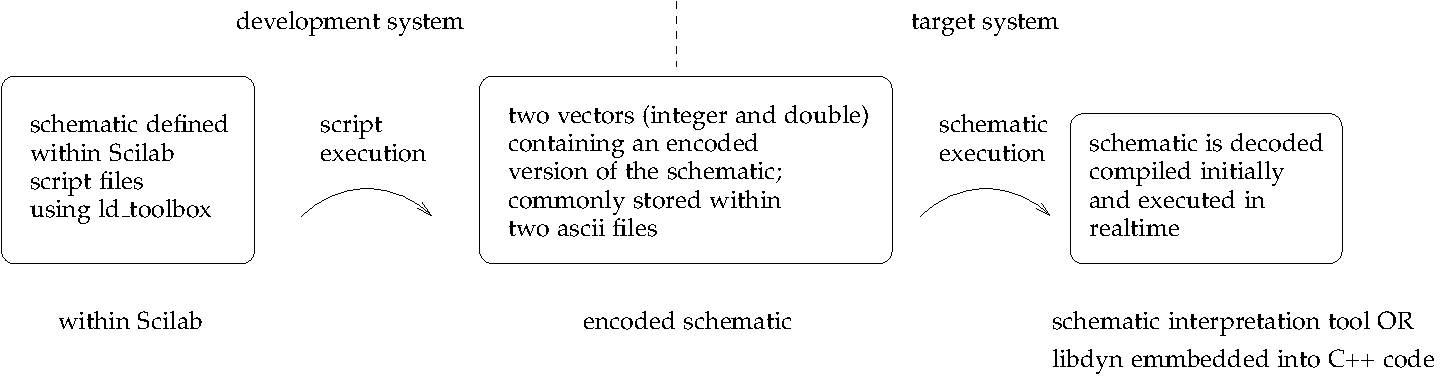
\includegraphics[width=0.98\linewidth]{pictures/principle.pdf} %width=0.8\columnwidth
\caption{Principle}
\label{fig:principle}
\end{figure}


\paragraph{Advantages}

\begin{itemize}
 \item No time needed to compile schematics through a C-Compiler -- they are internally interpreted just before execution. So there is no need to have a running (cross-) compilation environment for the target system for development of new schematics. Its needed only once to compile the library.
 \item Quick and easy integration of dynamic structures like control, digital signal processing and other algorithms into C/C++ - Code.
 \item schematic development is done within Scilab, thus controllers designed can be directly exported schematics that are executed within C/C++ - Code
 \item As schematics are described by Scilab function calls their structure can easily switched depending on arbitrary conditions. For example one schematic and also one C/C++ - program can be used to realise different experiments like identification- or control experiments, which are switched depending on the users decision.
 \item Schematics may be managed by subversion etc.
 \item Since it is only necessary to execute one Scilab-Script it is very fast to change parameters, transfer functions and even whole samples that are played in the simulation.
 \item Different events for block activation are possible.
\end{itemize}

\paragraph{Disadvantages}

\begin{itemize}
 \item Only time discrete blocks (may be changed by introducing a solver)
 \item Block can not generate events (at the moment).
 \item Less blocks than they can be found in Scicos or Simulink. Though it may be possible to use Scicos-Blocks if there was an interface. It is also easy to set-up own blocks.
 \item No GUI
\end{itemize}

\paragraph{Future extensions}

\begin{itemize}
  \item Schematics can be changed at runtime. This way an high level controller coded in C/C++ or even scilab choosing the lower level controller would be possible. Already possible but not in an elegant way.
  \item Port to run on a mC. It would then be possible to program new control structures without reflashing - only uploading a new schematic into ram is needed.
\end{itemize}


\section{Defining a schematic using Scilab commands}

\subsection{Blocks and connections}

Each schematic is based on one or more blocks that perform basic functionality like summation, filtering, multiplication and so on. Each block takes may take any number of input signals, which may be also vectorial signals. Additionally each block may have multiple output ports -- signal sources. Here is a basic definition of an block within Scilab:

\begin{verbatim}
  [sim, y] = ld_gain(sim, events, u, 1.5);
\end{verbatim}

This line would create a new block taking one input u multiplying it by $1.5$ and providing the result y via its output. The used signals u and y are represented by Scilab variables. They are somewhat special because they only refer to an signal and do only contain information about the source of the referred signal.
The identifier \texttt{sim} is an instance of an object that refers to the schematic to which the block should be added. Details are described later on. The second argument event contains information on which events (in a timely manner) should be directed to the block. Again, the details are described later on.
In order to connect further blocks the variable y could be used as an input for one or more blocks:

\begin{verbatim}
[sim, y_cut] = ld_sat(sim, event, y, -1, 1);
\end{verbatim}

Its also possible to combine certain blocks to a new block to gain some advance reusable functionality by defining a new Scilab function:

\begin{verbatim}
function [sim,y] = add_ofs(sim, events, u, ofs)
  [sim,ofs_const] = libdyn_new_blk_const(sim, events, ofs);
  
  [sim,y] = ld_add(sim, events, list(u,0, ofs_const,0), [1,1]);
endfunction
\end{verbatim}

Now, the new function can be used in the same manner as the predefined blocks:

\begin{verbatim}
[sim,y_cut_ofs] = add_ofs(sim, events, y_cut, 1);
\end{verbatim}

\section{Feedback loops}

At first consider this example:

\begin{verbatim}
function [sim, x,v] = oscillator(u)
    // create a feedback signal
    [sim,x_feedback] = libdyn_new_feedback(sim);

    // use this as a normal signal
    [sim,a] = ld_add(sim, defaultevents, list(u, x_feedback), [1, -1]);
    [sim,v] = ld_ztf(sim, defaultevents, list(a), 1/(z-1) * T_a ); // Integrator approximation
    [sim,x] = ld_ztf(sim, defaultevents, list(v), 1/(z-1) * T_a ); // Integrator approximation  
    
    // feedback gain
    [sim,x_gain] = ld_gain(sim, defaultevents, list(x), 0.6);
    
    // close loop x_gain = x_feedback
    [sim] = libdyn_close_loop(sim, x_gain, x_feedback);
endfunction
\end{verbatim}

Since the signal \texttt{x\_feedback}, which is used for feedback, is defined later on relative to the usage in the Scilab script, a provisional symbol has to be created by the command

\begin{verbatim}
[sim, x_feedback] = libdyn_new_feedback(sim);
\end{verbatim}

This creates a new signal x\_feedback that has no source for now. Its possible to use it as input for a block\footnote{Due to a limitation, at the time of writing it is only possible to connect one block}.

Later on, to assign a real signal to x\_feedback libdyn\_close\_loop is used:

\begin{verbatim}
[sim] = libdyn_close_loop(sim, x_gain, x_feedback);
\end{verbatim}

\subsection{events}

In every simulation up to 32 events are available, that are triggered by the C/C++ environment. Each block has one or more event inputs. To register certain events for a particular block most block-generating functions require a list of events to use. This list is represented by an integer vector, whereby the n-th element defines the event number for the n-th event input of the block. In the examples above this list was called \texttt{defaultevents}, which is commonly set to the vector \texttt{[0]} and denotes one regular occurring event. As an example, the list \texttt{[0,2,3]} registers three events to a block: The first is event 0, the second 2 and the last one is 3.
Events are used to update the states of the blocks or to fulfill special behavior like resetting the states, start/stop of a sampled sequence etc.

\subsection{Setting up a new schematic}

A new schematic is defined through a Scilab function:

\begin{verbatim}
function [sim, outlist] = schematic_fn(sim, inlist)
  [sim,u] = ld_const(sim, defaultevents, 1);
  
  [sim, x,y] = damped_oscillator(u);
  
  [sim] = ld_printf(sim, defaultevents, x, "x = ", 1);
  
  // save result to file
  [sim, save0] = libdyn_dumptoiofile(sim, defaultevents, "result.dat", list(x));
  
  // output of schematic
  outlist = list(x);
endfunction
\end{verbatim}

A schematic may have multiple input and output ports, which may be used as an interface to the users C/C++ - Code (see section \ref{sec:embeding}).

With help of the following Scilab code the schematic is generated and saved to disk:  

\begin{verbatim}
// defile events
defaultevents = [0]; // main event

// set-up schematic by calling the user defined function "schematic_fn"
insizes = [1,1]; outsizes=[1];
[sim_container_irpar, sim]=libdyn_setup_schematic(schematic_fn, insizes, outsizes);



//
// Save the schematic to disk (possibly with other ones or other irpar elements)
//

parlist = new_irparam_set();

// pack simulations into irpar container with id = 901
parlist = new_irparam_container(parlist, sim_container_irpar, 901);

// irparam set is complete convert to vectors
par = combine_irparam(parlist);

// save vectors to a file
save_irparam(par, 'oscillator.ipar', 'oscillator.rpar');

// clear
par.ipar = [];
par.rpar = [];
\end{verbatim}

The function \texttt{libdyn\_setup\_schematic} calls the defining function of the schematic and encodes the blocks parameters and the connections between blocks into two parameter vectors (integer and real values). This encoded information is stored within an irparm-set (integer and real parameter set), whereby the id 901 is assigned to the schematic, by the function \texttt{new\_irparam\_container}. During this process may other schematics with different ids may also be added to be stored in the same irparam-set. Lastly, the parameter sets are calculated and stored into two files for the integer and real part respectively.

% 
% \subsection{Some advanced methods}
% 
% 
% Saving a signal to a file:
% 
% \begin{verbatim}
%   sim=libdyn_dumptoiofile(sim, defaultevents, "Theta.dat", Theta);
% \end{verbatim}

% Play a sequence defined by a Scilab vektor:

% \begin{verbatim}
%   sequence = 1:0.01:100;
%   initial_play = 1;
%   [sim,sequence] = libdyn_new_blk_play(sim, [defaultevents], sequence, initial_play); 
% \end{verbatim}



\section{Embedding into C++ Code}
\label{sec:embeding}

Setting up a new libdyn instance with two input and two outputs each of size one:

\begin{verbatim}  
  int insizes[] = {1,1};
  int outsizes[] = {1,1};
 
  libdyn * simbox = new libdyn(2, insizes, 2, outsizes);
\end{verbatim}


setting up simulation input variables:

\begin{verbatim}
  struct {
    double r;
    double y;
  } acc_inputs; // sample input variables
  
  simbox->cfg_inptr(0, &acc_inputs.r); // set the first input to acc_inputs.r
  simbox->cfg_inptr(1, &acc_inputs.y); // set the second input to acc_inputs.y
\end{verbatim}

load a scematic or a set of multiple ones from two files generated by scilab:

\begin{verbatim}
  int *ipar_cpy; // pointer to integer parameter list
  double *rpar_cpy; // pointer to double parameter list
  int Nipar;  // length of ipar list
  int Nrpar;  // length of rpar list
    
  char *fname_i = "ldtest.ipar";
  char *fname_r = "ldtest.rpar";
  
  irpar_load_from_afile(&ipar_cpy, &rpar_cpy, &Nipar, &Nrpar, fname_i, fname_r); 
\end{verbatim}

compile schematic that is refered to by \texttt{schematic\_id} - this was defined in scilab code:
%\textrm{schematic_id} 

\begin{verbatim}
  int schematic_id = 901;
  err = simbox->irpar_setup(ipar_cpy, rpar_cpy, schematic_id);
  if (err == -1) { 
      // There may be some problems during compilation. 
      // Errors are reported on stdout
    printf("Error in libdyn\n");
    exit(1);
  }
\end{verbatim}

periodically calculation of outputs:

\begin{verbatim}
  acc_inputs.r = 0.3; acc_inputs.y = 0.6; // modify inputs

  int update_states = 0;
  simbox->simulation_step(update_states);

  double output1 = simbox->get_skalar_out(0);
  double output2 = simbox->get_skalar_out(1);  
\end{verbatim}

Periodical state update, with the possiblilty to trigger events:

\begin{verbatim}
    int eventmask = (1 << 0) +  // event number 0; alwas triggered
                    (low_freq_update << 1);  // another event number 1 
                                             // low_freq_update is 
                                             // either 1 or 0

    simbox->event_trigger_mask(eventmask);
    
    int update_states = 1;
    simbox->simulation_step(update_states); 
\end{verbatim}

close simulation and call destroy flag of all blocks:

\begin{verbatim}
  simbox->destruct();
\end{verbatim}

\section{Modules}

The whole space of blocks and functionality of this Toolbox is divided into several modules, which can be found in the \texttt{modules/} subdirectory.

\subsection{Interfacing functions}

Interfacing functions are Scilab functions, which define a certain block including its parameters. Each computational function should have at least one or more interfacing functions. TODO.

\subsection{Computitional function structure}

The computational functions are very similar in their structure compared to Simulink S-functions or Scicos computational functions. Though there are some additional features e.g. a flag for resetting internal states.

Plenty of rather simple examples for blocks are available within the \texttt{basic\_ldblocks} module. The file \texttt{basic\_ldblocks.c} contain the computational functions  and \texttt{scilab\_loader.sce} contains the corresponding interfacing functions for scilab.
To get an impression a computational function of a static block could look like:

\begin{verbatim}
int compu_func_sat(int flag, struct dynlib_block_t *block)
{
  int Nout = 1;  int Nin = 1;

  double *inp1;  double *out;	

  double *rpar = libdyn_get_rpar_ptr(block);
  double min = rpar[0];  double max = rpar[1];

  switch (flag) {
    case COMPF_FLAG_CALCOUTPUTS:
      inp1 = (double *) libdyn_get_input_ptr(block,0);
      out = (double *) libdyn_get_output_ptr(block,0);
      
      *out = *inp1;
      
      if (*out < min)
        *out = min;
      if (*out > max)
        *out = max;
      
      return 0;
      break;
    case COMPF_FLAG_UPDATESTATES:
      return 0;
      break;
    case COMPF_FLAG_CONFIGURE:  // configure
      libdyn_config_block(block, BLOCKTYPE_STATIC, Nout, Nin, (void *) 0, 0); 
      libdyn_config_block_input(block, 0, 1, DATATYPE_FLOAT); // in, intype, 
      libdyn_config_block_output(block, 0, 1, DATATYPE_FLOAT, 1);

      return 0;
      break;
    case COMPF_FLAG_INIT:  // init
      return 0;
      break;

    case COMPF_FLAG_DESTUCTOR: // destroy instance
      return 0;
      break;
  }
}
\end{verbatim}


The following flags are available:

\begin{itemize}
 \item \texttt{COMPF\_FLAG\_CONFIGURE}: Configure Blocks input sizes and types. DO NOT allocated memory or initialise hardware/ports etc.
 \item \texttt{COMPF\_FLAG\_INIT}: Called before simulation starts. Allocate memory; initialise hardware. If in this case the computational function returns -1, then the initialisation of the simulation is aborted and all blocks previously set-up will be destructed.
 \item \texttt{COMPF\_FLAG\_DESTUCTOR}: Destruct block instance.
 \item \texttt{COMPF\_FLAG\_CALCOUTPUTS}: Calculate outputs.
 \item \texttt{COMPF\_FLAG\_UPDATESTATES}: Update states.
 \item \texttt{COMPF\_FLAG\_PREPARERESET}: Prepare a statereset. (e.g. fetch the inputs  for storage)
 \item \texttt{COMPF\_FLAG\_RESETSTATES}: Reset the block to the initial state: Internal states as well as the output buffers are should be re-initialised. (This flag is an enormously helpful mechanism because it alows to completely reset nested simulations)
 \item \texttt{COMPF\_FLAG\_RELOAD\_IRPAR}: Not available for now. Called after new irpar parameters have been loaded.
 \item \texttt{COMPF\_FLAG\_PRINTINFO}: Print information about block instance on stdout.
\end{itemize}

During \texttt{COMPF\_FLAG\_CONFIGURE} the block has to be configured, which means that port numbers are assigned and allocated. Additionally the block type (dynamic or static has to be chosen). The function \texttt{libdyn\_config\_block} is responsible for both parts.

\begin{verbatim}
void libdyn_config_block(struct dynlib_block_t *block, int block_type, 
                         int Nout, int Nin, void *work, int own_outcache);
\end{verbatim}

First decide on the type of the block (\texttt{BLOCKTYPE\_STATIC} or \texttt{BLOCKTYPE\_DYNAMIC}), the number of in- and out-ports, a possible instance pointer, and whether memory for the output buffers is provided by the block (\texttt{own\_outcache} equals 1) or by the simulation system (\texttt{own\_outcache} equals 0). If unsure chose zero.


Then each input ports has to be configured. One input port \texttt{in} is configured to be of size \texttt{len}-Elements of \texttt{datatype} by the following call:

\begin{verbatim}
int libdyn_config_block_input(struct dynlib_block_t *block, int in, 
                              int len, int datatype);
\end{verbatim}

In an analog way this must be done for the outputs. Additionally the static dependence of an output on any input has to be marked by \texttt{dinput\_dependence = 1}

\begin{verbatim}
int libdyn_config_block_output(struct dynlib_block_t *block, int out, 
                               int len, int datatype, int dinput_dependence);
\end{verbatim}

Possible Datatypes are (others may follow):

\begin{itemize}
 \item \texttt{DATATYPE\_FLOAT} 
 \item \texttt{DATATYPE\_INT}
 \item \texttt{DATATYPE\_BOOLEAN}
\end{itemize}

You can also configure a work pointer by the macro:

\begin{verbatim}
 libdyn_set_work_ptr(block, work_);
\end{verbatim}

If it was chosen to allocate own output memory (\texttt{own\_outcache} = 1) you have to tell the library about it for each output port:

\begin{verbatim}
 void libdyn_config_outcache(struct dynlib_block_t *block, int Nout,  void *data);
\end{verbatim}



\paragraph{Pitfalls}

\begin{itemize}
 \item Never call \texttt{libdyn\_get\_input\_ptr} before the in or outputs are configured.
\end{itemize}




\section{Basic Schematic Set-up OLD STYLE}

Setting up a new simulation schematic:

\begin{verbatim}
  sim = libdyn_new_simulation([], []);
  defaultevents = [0];
  someotherevent = [1]; 
\end{verbatim}

Give all inputs a name referred by Scilab variables \texttt{phi} and \texttt{Theta} (at the moment this is not very nice but this will change in future):

\begin{verbatim}
  [simulation_inputs] = libdyn_get_input_signals(sim);
  
  // Give inputs a name
  [sim,interf1] = libdyn_new_interface(sim, defaultevents, 1);
  [sim,phi] = libdyn_conn_equation(sim, interf1, list(simulation_inputs, 0)); // port 0
  [sim,interf4] = libdyn_new_interface(sim, defaultevents, 1);
  [sim,Theta] = libdyn_conn_equation(sim, interf4, list(simulation_inputs, 1)); // port 1
\end{verbatim}

creating a new transfer function block, that is updated as a \texttt{defaultevents}-Event occurs:

\begin{verbatim}  
  [sim,tf_int] = libdyn_new_blk_zTF(sim, defaultevents, 1/(z-1));
\end{verbatim}

this block is then connected to signal \texttt{phi}, while the output is named \texttt{phi\_int}:

\begin{verbatim}
  [sim,phi_int] = libdyn_conn_equation(sim, tf_int, list(phi, 0));
\end{verbatim}

Blocks can also have multiple input ports:

\begin{verbatim}
  [sim,sum] = libdyn_new_blk_sum(sim, defaultevents, 1, -1);
  [sim,phi_int_minus_phi] = libdyn_conn_equation(sim, sum, list(phi_int, 0, phi, 0));
\end{verbatim}

connecting outputs and return signals to C:

\begin{verbatim}
   sim = libdyn_connect_extern_ou(sim, phi_int_minus_phi, 0, 0); // output port 0
   sim = libdyn_connect_extern_ou(sim, Theta, 0, 1); // output port 1
\end{verbatim}


\paragraph{Using events}

Every Block is initialised with a eventvector defining events that this block listens to. Every entry registers the block to an event referred by the value of this entry. The Block accesses these events in the same order as the events are referred in the eventvector. 

%For example if one block listens to its second event input it will 

Events are generated by setting an event mask in C-Code.



% 
% 
% \begin{appendix}
% 
% \begin{thebibliography}{99999}             % Hier beginnt das Literaturverzeichnis
% 
% \bibitem{hill1938}
% AV Hill,
% \newblock {\it The heat of shortening and the dynamic constants of muscle,}
% \newblock 1938.
% 
% 
% \end{thebibliography}
% \end{appendix}
% 


\end{document}
